\documentclass[10pt,draftclsnofoot,onecolumn, compsoc]{IEEEtran}
\usepackage{geometry}
\geometry{textheight=9.5in, textwidth=7in}
\usepackage{graphicx}
\usepackage{url}
\usepackage{setspace}
\usepackage{hyperref}
\usepackage{listings}
\usepackage{color}
\usepackage{tikz}
\usetikzlibrary{positioning}


\singlespacing
\setcounter{tocdepth}{5}
\setcounter{secnumdepth}{5}


\newcommand{\cred}[1]{{\color{red}#1}}
\newcommand{\cblue}[1]{{\color{blue}#1}}

\lstdefinestyle{customc}{
  belowcaptionskip=1\baselineskip,
  breaklines=true,
  frame=L,
  xleftmargin=\parindent,
  language=C,
  showstringspaces=false,
  basicstyle=\footnotesize\ttfamily,
  keywordstyle=\cred,
  identifierstyle=\cblue,
  stringstyle=\color{orange},
}


%% The following metadata will show up in the PDF properties
% \hypersetup{
%   colorlinks = false,
%   urlcolor = black,
%   pdfauthor = {\name},
%   pdfkeywords = {cs444 ``operating systems'' files filesystem I/O},
%   pdftitle = {CS 444 Project 2: I/O Elevators},
%   pdfsubject = {CS 444 Project 2},
%   pdfpagemode = UseNone
% }

\begin{document}
%\title{Team 13-03}
%\author{Joseph Struth  |  Josh Asher  |   Bryan Liauw}
%\date{}
%\maketitle
\begin{titlepage}
	\centering
	{\scshape\LARGE Team 13-03 \par}
	\vspace{1cm}
	{\scshape\Large Joseph Struth  |  Josh Asher  |   Bryan Liauw\par}
    \vspace{1cm}
    	{\scshape\Large Project 2: I/O Elevators \par}
	\vspace{1.5cm}
	{\huge\bfseries CS444\par}
	\vspace{2cm}
	{\Large\itshape Spring 2017\par}
	\vspace{4cm}
	{\large Abstract\par}
	\vspace{1cm}
	Our second project in this class involves implementing our own version of the LOOK I/O scheduler in the Yocto linux kernel, based on the No-op scheduler. This project gives us a much closer look at how requests are handled and dispatched at the kernel level.
	This document takes you through the process of designing and implementing our SSTF algorithm. Also attached is the second concurrency problem, the Dining Philosophers problem.
	\vfill

% Bottom of the page
	{\large \today\par}
\end{titlepage}

\section{Project 2 Questions}
\subsection{Question 1}
The main point of this assignment is to take our understanding of schedulers from a broad definition of round robin scheduling to an understanding of I/O Scheduling and how to implement it at the kernel level. This project also teaches us how to edit the menuconfig of a linux kernel. 
\subsection{Question 2}
Before we could solve this problem we had to understand it, and this is reflected in our work log. To design the algorithm for the \texttt{sstf-iosched.c} we had to first research and understand the \texttt{noop-iosched.c}. This involved also looking into the underlying data structures used in \texttt{noop-iosched} and other areas through out the kernel, mainly the \texttt{request\_queue}, \texttt{request}, and \texttt{elevator\_queue} structures. Next after we had individually researched the scheduler we were able to communicate and discuss which functions we actually needed to implement. At first we tried modifying both \texttt{sstf\_dispatch\_request} and \texttt{sstf\_add\_request}, until we realized how they get added to the queue is where the implementation of the algorithm will be done (Thanks to Brian for pointing this out before we were told in class). The No operation scheduler was our main reference in this assignment, and the C-LOOK scheduler we were implementing is very similar. So we started with renaming all no-op functions to sstf (shortest seek time first) \cite{celis_gonzales_2014}. To implement LOOK, the \texttt{sstf\_add\_request} function will have to be modified. Add request will be modified to, if the request queue is not empty it will look for the closest request that is larger than the current requests position. This is done to, in the case of a physical hard drive with a read and write it will try and go toward greater sectors until the queue is empty. Our request data structure is below, with utilizes Linux's built in kernel implementation of a circular double linked-list.
\begin{lstlisting}[language=C, style=customc]
struct sstf_data {
        struct list_head queue;
};
\end{lstlisting}
C-LOOK and SSTF are called elevator algorithms because they will service all requests in one direction on the disk. It won't reverse the direction of the read or write like LOOK would. C-LOOK will go in one direction, until there are no more requests then it will begin the process again.
Next we began a period of trial and error trying to figure out where in the kernel configuration needed to be changed to add the LOOK scheduler.
\subsection{Question 3}
To test our SSTF scheduler, after configuring the new scheduler and running the virtual machine we used a script to generate random file read and write I/O. Using the kernel print function \texttt{printk()} we were able to see sector number from the read and write requests. We knew the scheduler worked as the sector numbers would increase with the amount of read and write requests that were processed. Below in Figure 1 is our graph of read and write operations with time on the x-axis and sector distance on the y axis.

\vspace{5mm} %5mm vertical space

Fig 1. SSTF Read and Write Operations
\centering
\begin{figure}[htb]
\begin{tikzpicture}
  \node (img1)  {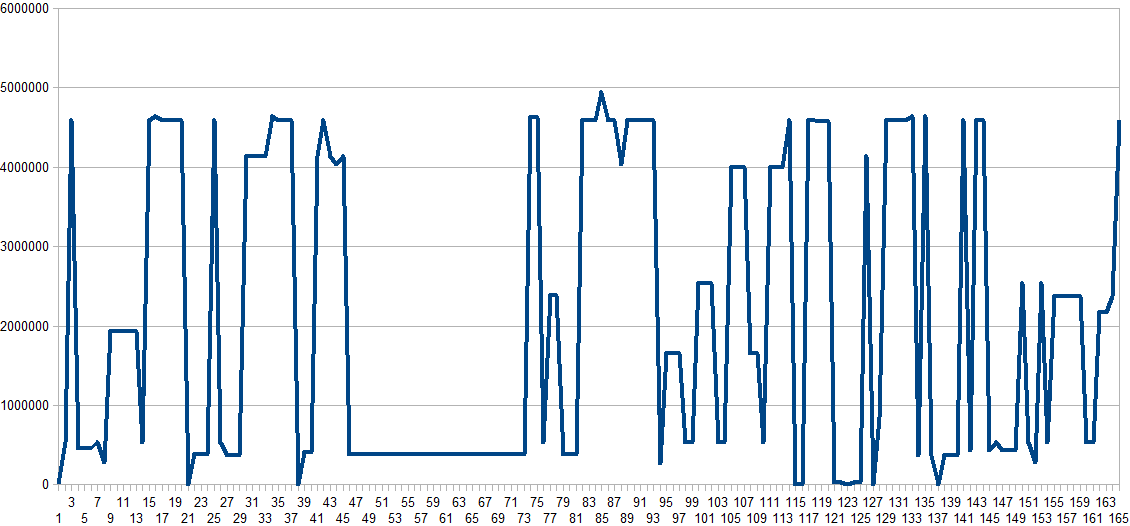
\includegraphics[scale=0.5]{Graph2}};
  \node[below=of img1, node distance=0cm, yshift=1cm,font=\color{blue}] {Time};
  \node[left=of img1, node distance=0cm, rotate=90, anchor=center,yshift=-0.7cm,font=\color{blue}] {Sector Distance};
\end{tikzpicture}
\centering
\end{figure}

\newpage
\subsection{Question 4}
In this project we learned a lot more about how I/O Schedulers operate and how to implement them. We also learned more about how to change components in the Linux kernel through modifying the configuration. It is surprising how a few lines of code in a scheduler can be so complicated and require a good amount of reading before any actual coding can be done! 

\section{Git Log}

\begin{tabular}{| l | l | p{15cm} |}\textbf{Detail} & \textbf{Author} & \textbf{Description}\\\hline
\href{https://github.com/struthj/CS444/commit/95f2f83c730dfb35f0292b3a825747fdde110c49}{95f2f83} & Joseph Struth & Started Concurrency 2 Dining Philosophers.\\\hline
\href{https://github.com/struthj/CS444-1303/commit/a933104c6c986f873737877b29bcf222933f805d}{a933104} & Joseph Struth & Created Team Git repository.\\\hline
\href{https://github.com/struthj/CS444-1303/commit/a176f8a30f2adef093bb56e16eb97c264fc956ec}{a176f8a} & Joseph Struth & Added concurrency 2 philosophers dining problem .\\\hline
\href{https://github.com/struthj/CS444-1303/commit/ec7c9692fc67d925772e42ce9317378f85fdb296}{ec7c969} & Joshua Asher & Added Basic sstf-iosched.c.\\\hline
\href{https://github.com/struthj/CS444-1303/commit/ec7c9692fc67d928f85fdb2965772e42ce931737}{ec7c988} & Joshua Asher & Added a little to the write up.\\\hline
\end{tabular}

\section{Work Log}

\begin{tabular}{| l | l | p{15cm} |}\textbf{Date} & \textbf{Author} & \textbf{Details}\\\hline
4-19-2017 & Joseph Struth & Started Concurrency 2 Assignment mostly finished.\\\hline
4-20-2017 & Joseph Struth & Finished Concurrency 2 with Help from Joshua Asher (for finding my segfault!).\\\hline
4-9-2017 & Joseph Struth & Fixed Resize for Concurrency 1 Assignment.\\\hline
4-27-2017 & Joseph Struth & Created group repository and cloned Yocto Kernel.\\\hline
5-2-2017 & Joshua Asher & Looked over kernel code and read to understand LOOP algorithm.\\\hline
5-3-2017 & Brian Liauw & Read to understand implementation .\\\hline
5-3-2017 & Brian Liauw Josh Asher & Found related subject example code to help understanding of assignment.\\\hline
5-3-2017 & Joseph Struth Josh Asher & Met in Library to work on assignment.\\\hline
5-4-2017 & Brian Liauw & Worked on Add request function.\\\hline
5-4-2017 & Joseph Struth & Wrote python test script for I/O.\\\hline
5-6-2017 & Joshua Asher & Worked on kernel config and scheduler.\\\hline
5-6-2017 & Brian Liauw Joshua Asher & Worked on compiling kernel with sstf scheduler.\\\hline
5-7-2017 & Joseph Struth & Started Write up questions, introduction, and work logs.\\\hline
5-8-2017 & Brian Liauw & Made patch file.\\\hline
5-7-2017 & All of us & Finalizing home work and tar balling so we can submit.\\\hline
\end{tabular}

\section{Bibliography}
\nocite{*}
\bibliographystyle{IEEEtran}
\bibliography{HW1Bibliography.bib}


\end{document}
